\chapter{計測結果}
\label{cha:result}
計測はbashのtimeコマンドを使用した。また、\cite{bash}を参考にシェルスクリプトを使用して計測の自動化を行った。また、以下の計測の時間単位は(s)である。
\section{フィボナッチ数列}
n番目のフィボナッチ数を求めるプログラムの実行速度をそれぞれ20回ずつ測定した。
計20回の結果の平均は図\ref{fig:f-average}となった。
また、計20回の結果の分散は図\ref{fig:f-dispersion}となった。
図\ref{fig:f-dispersion}をから分散は非常に小さいことが読み取れる。
どのスクリプト言語も導出するフィボナッチ数が大きくなるほど実行時間が伸びる傾向にある。
図\ref{fig:f-average}を見ると導出するフィボナッチ数が20回までの間はrubyが最も早く動作することがわかった。
しかし、導出するフィボナッチ数が増加するのに伴って、node.jsの処理速度の速さが目立つようになった。
また、40個目のフィボナッチ数を求めるのが最も遅かったのはPython3で約30秒という結果になった。

\section{円周率の算出}
ライプニッツ級数を使った円周率を求めるプログラムの実行速度をそれぞれ20回ずつ測定した。
どのスクリプト言語も導出した円周率に差異はないが、プログラムの実行時間に差があった。
計20回の結果の平均は図\ref{fig:p-average}となった。
また、計20回の結果の分散は図\ref{fig:p-dispersion}となった。
図\ref{fig:p-dispersion}をから分散は非常に小さいことが読み取れる。
フィボナッチ数列の結果とは違い、実行した回数に限らずPHPが最も早く処理をすることができた。
また今回の測定ではpython3は最も遅く、PHPの約200倍の時間がかかったことがわかる。

\section{正規表現}
正規表現を使ったURLを検出するプログラムの実行速度をそれぞれ20回ずつ測定した。
どのスクリプトも同じようにURLを検出した。それぞれのプログラムの実行時間に差があった。
計20回の結果の平均は図\ref{fig:s-average}となった。
また、計20回の結果の分散は図\ref{fig:s-dispersion}となった。
図\ref{fig:s-dispersion}をから分散は非常に小さいことが読み取れる。
図\ref{fig:s-dispersion}からnode.jsとPHPが非常に高速であることが読み取れる。
また、Python3も十分に速くフィボナッチとや円周率よりと比べると良い結果になっていることがわかる。
今回計測した中で最も遅かったのはrubyの約23秒だった。


\clearpage
\begin{figure}[tb]
    \centering
    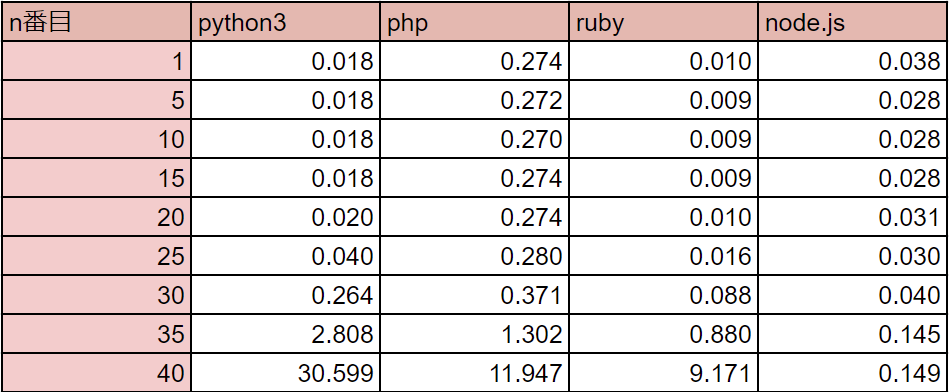
\includegraphics[width=14.5cm,keepaspectratio]{figure/f-average.PNG}
    \caption{フィボナッチ数列 平均}
    \label{fig:f-average}
\end{figure}

\begin{figure}[tb]
    \centering
    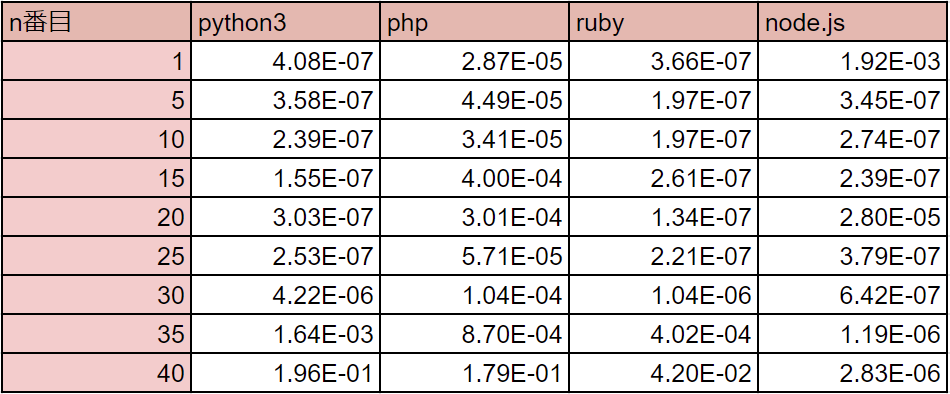
\includegraphics[width=14.5cm,keepaspectratio]{figure/f-dispersion.PNG}
    \caption{フィボナッチ数列 分散}
    \label{fig:f-dispersion}
\end{figure}

\clearpage

\begin{figure}[tb]
    \centering
    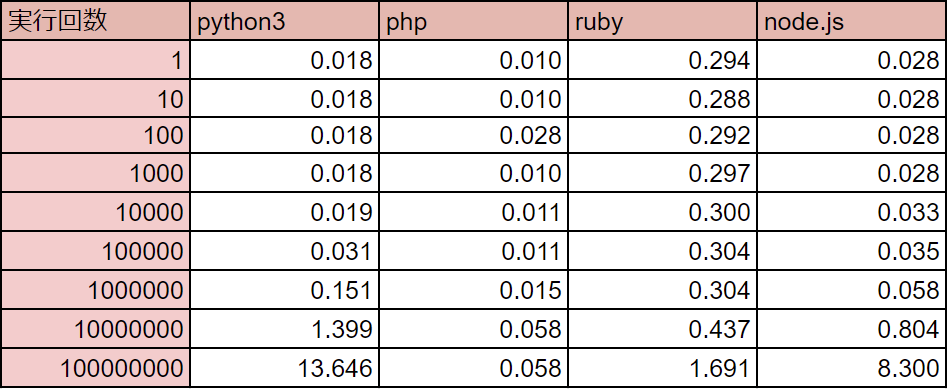
\includegraphics[width=14.5cm,keepaspectratio]{figure/p-average.PNG}
    \caption{円周率の算出 平均}
    \label{fig:p-average}
\end{figure}

\begin{figure}[tb]
    \centering
    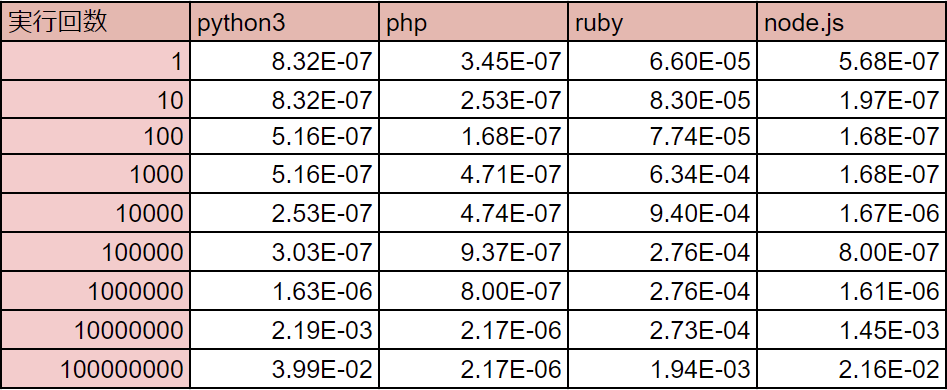
\includegraphics[width=14.5cm,keepaspectratio]{figure/p-dispersion.PNG}
    \caption{円周率の算出 分散}
    \label{fig:p-dispersion}
\end{figure}

\clearpage

\begin{figure}[tb]
    \centering
    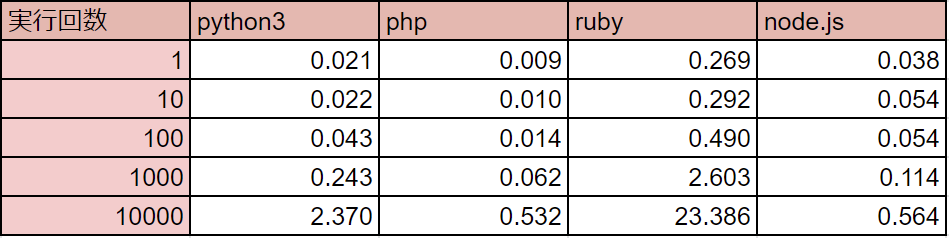
\includegraphics[width=14.5cm,keepaspectratio]{figure/s-average.PNG}
    \caption{正規表現 平均}
    \label{fig:s-average}
\end{figure}

\begin{figure}[tb]
    \centering
    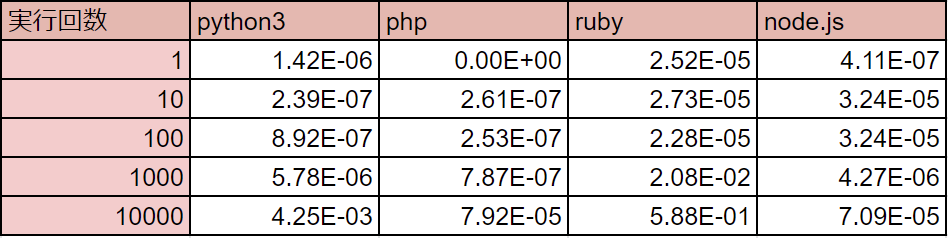
\includegraphics[width=14.5cm,keepaspectratio]{figure/s-dispersion.PNG}
    \caption{正規表現 分散}
    \label{fig:s-dispersion}
\end{figure}
